\section{Results}

Let's explore the test phase and see the results in detail. Initially we ran debug tests on our personal PCs in order to easily modify the code, these starting tests and the tests utilized to determine the right value for the many defined constants are not shown here. 

All the tests shown below were performed on a single more powerful machine that has enabled us to work with much larger data in less time. The machine used is composed of two Xeon processors for a total of 16 cores 2.80 Ghz and 48 Gb of RAM.

The tests were performed on a growing number of scans, each containing a maximum of 50 lines from which we extracted the words that represent the states. For each set of scans we present three possible distances calculation: only LCS, only L1 (Euclidean distance) and LCS and L1 combined together through the formula presented in Section 5.

\vspace{3mm}

\begin{itemize}
\item \textbf{Estimated words (E)}: the number of words estimated on the basis of the number of scans(50x).
\item \textbf{Extracted words (W)}: the number of words actually mined and processed, as well as the corresponding percentage.
\item \textbf{Number of clusters (C)}: the number of clusters created in process.
\item \textbf{Running time (T)}: the total execution time, in seconds.
\item \textbf{Average precision (AP)}: the accuracy of the results, the average accuracy of clusters.
$$Precision_{average} = \frac{\sum_i P_i}{N_c}$$
where $P_i$ is the precision of cluster $i$ and $N_c$ is the number of clusters. 
\item \textbf{Precision (P)}: the accuracy of the results, the average accuracy of individual clusters weighted with the number of words.
$$Precision = \frac{\sum_i P_i * n_i}{N_w}$$
where $P_i$ is the precision of cluster $i$, $n_i$ is the number of words in cluster $i$ and $N_w$ is the number of words. 
\end{itemize}

In the next table are shown the main results of the tests. 

\begin{table}[H]
\centering
\footnotesize
\begin{tabular}{|l | c | c | c | c | c | c |} 
 \hline 
 & \textbf{E} &  \textbf{W} & \textbf{C} & \textbf{T} & \textbf{AP} & \textbf{P} \\ [0.5ex] 
 \hline\hline
%% label & estimated words & extracted words & clusters & time & precision %%
16 scans (L1) & 800 & 550 & 55 & 15.52 & 65.06 & 58.00\\ 
16 scans (LCS) & 800 & 550 & 71 & 44.39  & 76.56 & 60.00\\ 
16 scans (LCS and L1) & 800 & 550 & 66 & 47.41 & 74.37 & 62.91\\ \hline
32 scans (L1) & 1600 & 800 & 67 & 38.58 & 59.85 & 52.87\\ 
32 scans (LCS) & 1600 & 800 & 92 & 94.54 & 72.97 & 55.50\\ 
32 scans (LCS and L1) & 1600 & 800 & 86 & 112.90 & 70.19 & 56.25\\ \hline
75 scans (L1) & 3750 & 2350 & 173 & 221.03 & 69.03 & 63.65\\ 
75 scans (LCS) & 3750 & 2350 & 189 & 1169.72 & 75.09 & 67.49\\ 
75 scans (LCS and L1) & 3750 & 2350 & 199 & 1203.28 & 78.01 & 71.16\\ \hline
130 scans (L1) & 6500 & 5050 & 425 & 5444.43 & 76.66 & 71.12\\ 
130 scans (LCS) & 6500 & 5050 & 441 & 5629.71 & 82.11 & 74.41\\ 
130 scans (LCS and L1) & 6500 & 5050 & 463 & 6729.62 & 84.87 & 77.94\\ \hline
500 scans (L1) & 25000 & 18146 & 3957 & 85545.11 & 90.66 & 77.89\\ 
500 scans (LCS) & 25000 & 18146 & 3316 &  76324.63 & 91.02 & 81.22\\ 
500 scans (LCS and L1) & 25000 & 18146 & 3941 & 138309.85\tablefootnote{During this test, the machine used was concurrently executing other tasks creating a bottleneck in the allotted memory, in all similar tests the time was in the order of 90k seconds.} & 92.27 & 82.14\\ 
 \hline
\end{tabular}
\caption{Main results}
\label{table:1}
\end{table}

As we can see in Table \ref{table:1} the number of extracted words is much lower than the estimated number of words. This is mainly due to the fact that not all census tables are completely filled: in some cases there are only a few lines or the states column was purposefully left blank. In other cases the absence of the state samples is due to errors occurring in the segmentation phase due to a wrong interpretation of the rows or the columns.

As we can see in Figure \ref{fig:precision} the accuracy of the cluster grows with the amount of words extracted. This phenomenon is due to the fact that Affinity Propagation works best with a large number of available data: the greater the number of words, the greater the chances of finding words similar between them, and then combine them within a single cluster.


\begin{figure}[H]
\centering
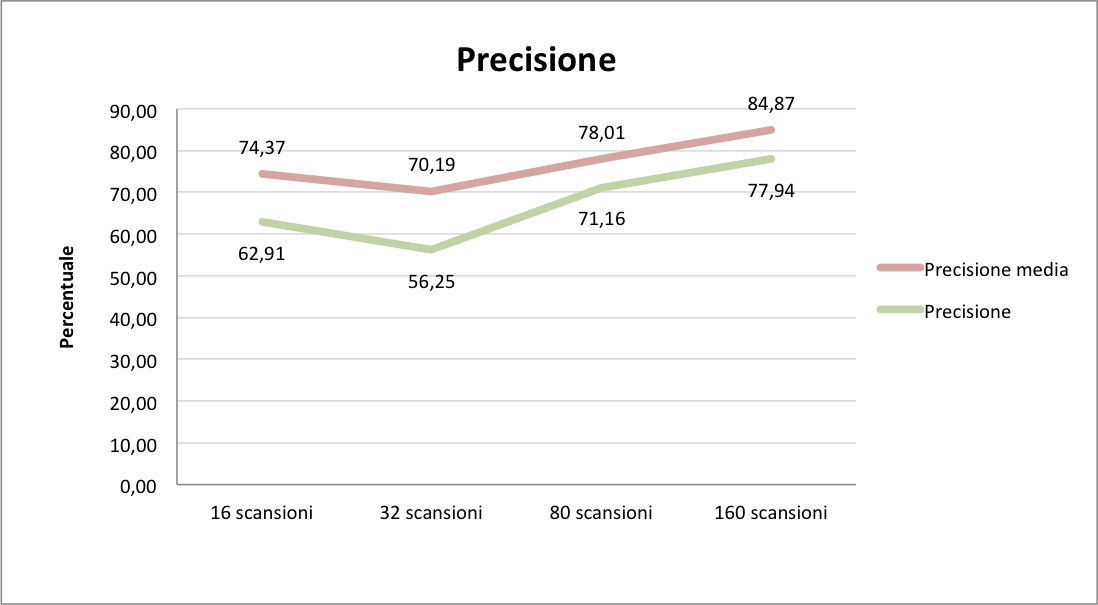
\includegraphics[width=0.7\textwidth]{images/precisione.png}
\caption{Clustering precision relative to the number of scans}
\label{fig:precision}
\end{figure}

In the next table are presented the results regarding the time needed for the calculations. The running time is divided mainly into three distinct categories corresponding to different phases of the process: time needed for the extraction of features, time needed for the creation of similarity matrix (calculation of distances) and time needed for the clustering.

\begin{itemize}
\item \textbf{Features extraction time}: the time, in seconds, required for features extraction from the words.
\item \textbf{Evaluating distances time}: the time, in seconds, required to generate the similarity matrix with the distances between all the words extracted.
\item \textbf{Clustering time}: the time, in seconds, required for the creation of clusters.
\item \textbf{Running time}: the total execution time, in seconds.
\end{itemize}

\begin{table}[H]
\centering
\footnotesize
\begin{tabular}{|l | c | c | c | c |} 
 \hline 
 & \multicolumn{1}{p{2cm}|}{\centering\bfseries Features extraction\\time (s)}&  \multicolumn{1}{p{2cm}|}{\centering\bfseries Evaluating distances\\time (s)} & \multicolumn{1}{p{2cm}|}{\centering\bfseries Clustering\\ time (s)} & \multicolumn{1}{p{2cm}|}{\centering\bfseries Total (s)} \\ [0.5ex] 
 \hline\hline
%% label & features & distances & clusters & total %%
16 scans (L1) & 6.81 & 5.02 & 3.69 & 15.52\\ 
16 scans (LCS) & 6.84 & 34.40 & 3.15 & 44.39\\ 
16 scans (LCS and L1) & 6.84 & 37.32 & 2.85 & 47.41\\ \hline
32 scans (L1) & 11.54 & 7.22 & 19.82 & 38.58\\ 
32 scans (LCS) & 11.27 & 74.72 & 8.55 & 94.54\\ 
32 scans (LCS and L1) & 11.34 & 89.96 & 11.60 & 112.90\\ \hline
75 scans (L1) & 33.65 & 69.00 & 118.38 & 221.03\\ 
75 scans (LCS) & 35.13 & 1002.63 & 131.96 & 1169.72\\ 
75 scans (LCS and L1) & 34.70 & 1070.92 & 97.66 & 1203.28\\ \hline
130 scans (L1) & 70.80 & 313.70 & 5059.93 & 5444.43\\ 
130 scans (LCS) & 68.17 & 4353.85 & 1207.69 & 5629.71\\ 
130 scans (LCS and L1) & 73.10 & 5608.82 & 1047.70 & 6729.62\\ \hline
500 scans (L1) & 289.33 & 4482.02 & 80773.76 & 85545.11 \\ 
500 scans (LCS) & 323.66 & 57699.51 & 18301.46 & 76324.63\\ 
500 scans (LCS and L1) & 403.41 & 61424.57 & $76481.87^5$ & $138309.85^5$\\ 
 \hline
\end{tabular}
\caption{Running time}
\label{table:2}
\end{table}

As we can see in Table \ref{table:2} the complexity is mainly due to the construction phase of the similarity matrix, that is the calculation of distances. This high operative cost occurs especially in calculating the LCS distance due to the fact that the structural strings of our words are very long and the cost of the algorithm is $O(nm)$, with $n$ and $m$ the lengths of the two strings, cost that must be considered in each comparison between couples of samples.

We sought long structural strings to obtain a deeper characterization of the words (and therefore make more accurate clustering), but this necessarily increases the calculation time.

\begin{figure}[!htbp]
\centering
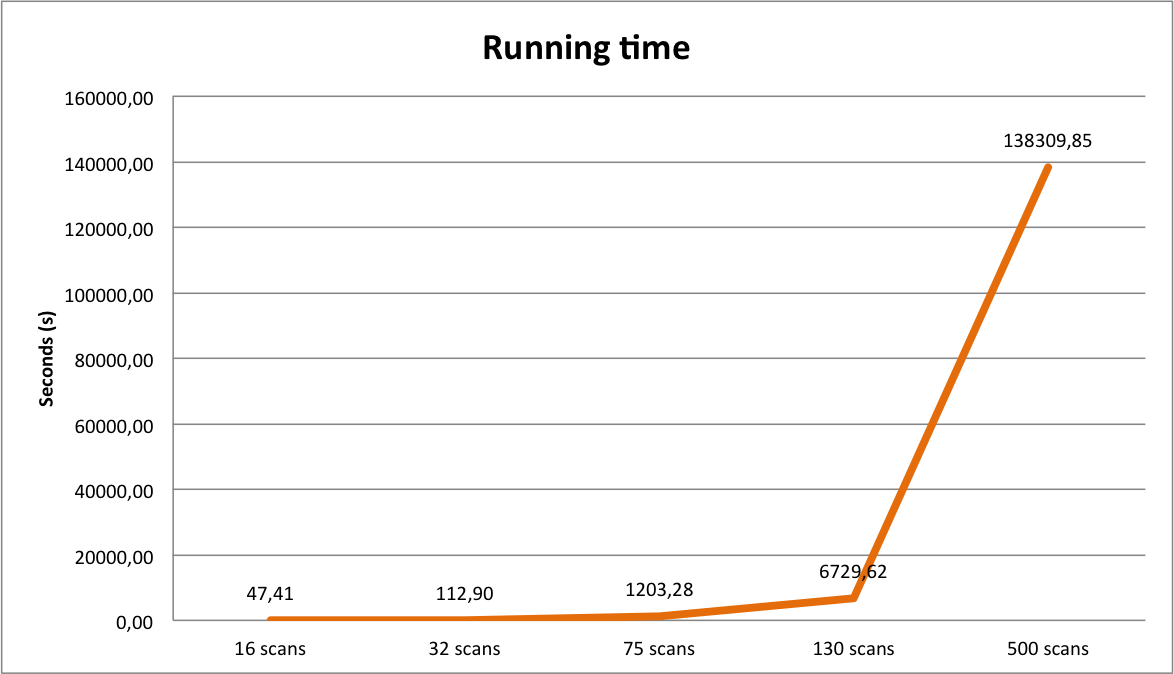
\includegraphics[width=0.7\textwidth]{images/esecuzione}
\caption{Running time relative to the number of scans}
\label{fig:time}
\end{figure}

A parameter to evaluate the goodness of our application relatively to the task can be the number of clusters that have the absolute precision, that is contain only similar elements that are properly classified(due to human error sometimes the words in the debug files suffer a faulty categorization).

In the following table are presented the number of clusters which respect the above property and the number of items that they contain. 

\begin{itemize}

\item \textbf{Correct clusters}: the number of clusters with absolute precision, therefore containing only words equal to each other.
\item \textbf{Correct words}: the number of words within the Correct clusters and their corresponding percentage respect to all the elements.
\item \textbf{Single clusters}: clusters containing only one word.
\item \textbf{Average words for correct non-single cluster} (\textbf{AWCC}): number of words in average in the correct clusters that do not contain a single element.
\end{itemize}

\begin{table}[H]
\centering
\footnotesize
\begin{tabular}{|l | c | c | c | c |} 
 \hline 
 & \multicolumn{1}{p{2cm}|}{\centering\bfseries Correct\\ clusters}&  \multicolumn{1}{p{2cm}|}{\centering\bfseries Correct\\words} & \multicolumn{1}{p{2cm}|}{\centering\bfseries Single\\clusters} & \multicolumn{1}{p{2cm}|}{\centering\bfseries AWCC} \\ [0.5ex] 
 \hline\hline
%% label & clusters & words & percentage %%
16 scans (L1) & 12 & 18 & 10 &  3.00\\ 
16 scans (LCS) & 33 & 44 & 29 & 2.75\\ 
16 scans (LCS and L1) & 25 & 45 & 18 & 6.43\\ \hline >>>CONTINUAMI
32 scans (L1) & 11 & 11 & 10 & xx.00\\ 
32 scans (LCS) & 39 & 48 & 36 &1.23\\ 
32 scans (LCS and L1) & 32 & 43 & 28 & 1.34\\ \hline
75 scans (L1) & 39 & 172 & 11 & 4.41\\ 
75 scans (LCS) & 78 & 265 & 43 & 3.40\\ 
75 scans (LCS and L1) & 77 & 316 & 43 & 4.10\\ \hline
130 scans (L1) & 138 & 651 & 23 & 4.72\\ 
130 scans (LCS) & 208 & 713 & 107 &  3.43\\ 
130 scans (LCS and L1) & 215 & 860 & 89 & 4.00\\ \hline
500 scans (L1) & 2854 & 7354 & 151 & 2.58\\ 
500 scans (LCS) & 2902 & 7423 & 163 & 2.56\\ 
500 scans (LCS and L1) & 3020 & 7616 & 145 & 2.52\\ 
 \hline
\end{tabular}
\caption{Correct clusters}
\label{table:3}
\end{table}
